%!TEX root=ast2016.tex

% \section{Empirical Study}
% \label{sec:empirical-study}

\section{Experimental Setup}
\label{sec:experimental-setup}

% TODO: Add in one introductory sentence to start off this section

\subsection{Relational Database Schemas}
\label{sec:subjects}

%!TEX root=../ast2016.tex

\begin{table}[t!]
	\caption{Schemas analysed in the empirical study} \label{tbl:study-schemas}
	\scriptsize
	\centering
	\scalebox{\tablescalefactor}{
		\begin{tabular}{l@{\hskip -5pt}rrrrrrrr}
			{Schema}           & \rot{Tables} & \rot{Columns} & \rot{Checks} & \rot{Foreign Keys} & \rot{Not Nulls} & \rot{Primary Keys} & \rot{Uniques} & \rot{$\sum$Constraints} \\ \hline
			ArtistSimilarity & 2 & 3 & 0 & 2 & 0 & 1 & 0 & 3 \\
			ArtistTerm & 5 & 7 & 0 & 4 & 0 & 3 & 0 & 7 \\
			BankAccount & 2 & 9 & 0 & 1 & 5 & 2 & 0 & 8 \\
			BookTown & 22 & 67 & 2 & 0 & 15 & 11 & 0 & 28 \\
			BrowserCookies & 2 & 13 & 2 & 1 & 4 & 2 & 1 & 10 \\
			Cloc & 2 & 10 & 0 & 0 & 0 & 0 & 0 & 0 \\
			CoffeeOrders & 5 & 20 & 0 & 4 & 10 & 5 & 0 & 19 \\
			CustomerOrder & 7 & 32 & 1 & 7 & 27 & 7 & 0 & 42 \\
			DellStore & 8 & 52 & 0 & 0 & 39 & 0 & 0 & 39 \\
			Employee & 1 & 7 & 3 & 0 & 0 & 1 & 0 & 4 \\
			Examination & 2 & 21 & 6 & 1 & 0 & 2 & 0 & 9 \\
			Flights & 2 & 13 & 1 & 1 & 6 & 2 & 0 & 10 \\
			FrenchTowns & 3 & 14 & 0 & 2 & 13 & 0 & 9 & 24 \\
			Inventory & 1 & 4 & 0 & 0 & 0 & 1 & 1 & 2 \\
			Iso3166 & 1 & 3 & 0 & 0 & 2 & 1 & 0 & 3 \\
			iTrust & 42 & 309 & 8 & 1 & 88 & 37 & 0 & 134 \\
			JWhoisServer & 6 & 49 & 0 & 0 & 44 & 6 & 0 & 50 \\
			MozillaExtensions & 6 & 51 & 0 & 0 & 0 & 2 & 5 & 7 \\
			MozillaPermissions & 1 & 8 & 0 & 0 & 0 & 1 & 0 & 1 \\
			NistDML181 & 2 & 7 & 0 & 1 & 0 & 1 & 0 & 2 \\
			NistDML182 & 2 & 32 & 0 & 1 & 0 & 1 & 0 & 2 \\
			NistDML183 & 2 & 6 & 0 & 1 & 0 & 0 & 1 & 2 \\
			NistWeather & 2 & 9 & 5 & 1 & 5 & 2 & 0 & 13 \\
			NistXTS748 & 1 & 3 & 1 & 0 & 1 & 0 & 1 & 3 \\
			NistXTS749 & 2 & 7 & 1 & 1 & 3 & 2 & 0 & 7 \\
			Person & 1 & 5 & 1 & 0 & 5 & 1 & 0 & 7 \\
			Products & 3 & 9 & 4 & 2 & 5 & 3 & 0 & 14 \\
			RiskIt & 13 & 57 & 0 & 10 & 15 & 11 & 0 & 36 \\
			StackOverflow & 4 & 43 & 0 & 0 & 5 & 0 & 0 & 5 \\
			StudentResidence & 2 & 6 & 3 & 1 & 2 & 2 & 0 & 8 \\
			UnixUsage & 8 & 32 & 0 & 7 & 10 & 7 & 0 & 24 \\
			Usda & 10 & 67 & 0 & 0 & 31 & 0 & 0 & 31 \\
			\hline
			{Total} & 172 & 975 & 38 & 49 & 335 & 114 & 18 & 554 \\
			\hline

		\end{tabular}
	}
\end{table}


\begin{itemize}
  \item 32 schemas
    \begin{itemize}
      \item 1 to 42 tables
      \item 3 to 309 columns
      \item 0 to 134 constraints
      \item Includes each of the types of constraint supported by \SchemaAnalyst (\PK, \FK, \NOTNULL, \UNIQUE and \CHECK constraints)
    \end{itemize}
  \item 3 DBMSs -- \Postgres, \HyperSQL (in-memory), \SQLite (in-memory)
  \item 30 repeated trials
  \item 2 techniques -- \Original and \VirtualMutationAnalysis
  \item Metrics -- time taken for mutation analysis, number of mutants, number of test cases
  \item Mention that the mutation scores of the Original technique are used to validate the results given by virtual mutation analysis, and that in every case the results were identical. (Possibly repeat this in the threats section?)
\end{itemize}

\subsection{Research Questions}
\label{sec:research-questions}

The experiments in this paper investigate three research questions, which we state in the following fashion.

\vspace{5pt}

\noindent
\textbf{RQ1 (Efficiency):} How does the time overhead of \VMA compare to the \Standard technique's cost, and how does
this vary depending on the DBMS in use?

\vspace{5pt}

\noindent
\textbf{RQ2 (Scalability):} How does the time savings from using \VMA scale when increasing either the number
of analysed mutants or the number of executed tests?

\vspace{5pt}

% can only analyse mutants for the same amount of time as the presented approach?

\noindent
\textbf{RQ3 (Effectiveness):} How does the mutation score of \VMA compare to the score of a time-constrained method that
is only permitted to run for as long as the virtual one?

\subsection{Methodology}
\label{sec:methodology}
For RQs 1 and 2, we ran the \Original technique and \vma 30 times each, for each of the schemas with each of the DBMSs, collating the time taken. For each run, we used a test suite automatically generated using a search-based technique with a unique random seed.

Details of the specific test suite generation algorithms used are detailed by McMinn \etal~\cite{McMinn2015}. We used the \AVM method as it is the most reliable automated technique for generating high levels of test coverage. The coverage criterion we used was a combination of ``ClauseAICC'', ``AUCC'' and ``ANCC'', which merges the strongest criteria for testing the integrity constraints of database schemas.

For RQ3, we then ran the \Original technique 30 times, but by performing mutation analysis by selecting mutants at random until each the time taken for the corresponding run of the 30 repetitions of \vma was exhausted.

We performed all experiments with our \SA tool \cite{Kapfhammer2013,Wright2014,McMinn2015},
compiled with the Java Development Kit 7 compiler and executed with the Linux version of the 64-bit Oracle Java 1.7 virtual machine. Experiments were executed on an Ubuntu 14.04 workstation, with a 3.13.0-44 GNU/Linux 64-bit kernel, a quad-core 2.4GHz CPU and 12GB RAM. All input (i.e., schemas) and output (i.e., data) files were stored on the local disk. We used the default configuration of \PostgreSQL version 9.3.5, \HyperSQL version 2.2.8 and \SQLite 3.8.2. \HyperSQL and \SQLite were used with ``in-memory'' mode enabled.

\subsection{Evaluation Metrics}
\label{sec:evaluation-metrics}

\subsection{Threats to Validity}
\label{sec:threats-to-validity}

% TODO: Explain that we check the mutation score to ensure that Standard and Virtual are the same!
% TODO: Reference the SSBSE 2015 paper that talks about transformation of the values; we also
% did this and we are certain that there is no difference (we also looked at different thresholds).

\section{Empirical Results}
\label{sec:empirical-results}

% PURPOSE: Compare the virtual mutation technique to the original one in terms of their execution time, showing that
% virtual mutation is often significantly faster than the standard approach to mutation analysis.

\subsection{Comparing Original and Virtual Mutation}
\label{sec:empirical-study-RQ-original-virtual-time}
% vim: ft=tex
%!TEX root=ast2016.tex

% PURPOSE: Discuss the trends in the first graph, sketching at a high level

\inlineheading{Comparing Standard and Virtual Mutation}~The box and whisker plots in Figure~\ref{fig:graphic_bwplot_schema_analysistime_org_vm} show the mutation analysis time for the two techniques across all of the relational schemas and the three DBMSs. This plot reveals that, when using the \HyperSQL~DBMS, the \virtual~method is faster than the \Original~one, especially for large schemas such as JWhoisServer. Since \Postgres~is a ``heavyweight'' disk-based DBMS, \vma~demonstrates much lower execution times than the \Original~method because it avoids database interactions. Yet, these plots show that the performance of the virtual approach is similar to the standard one when mutation analysis runs on the high-performance \sqlite~DBMS.

% PURPOSE: Analyse the trends further through the statistical analysis and the effect size computations. For effect
% sizes, make sure to comment on the fact that we did thresholding of the scores.

The statistical tests and effect size calculations confirm the trends evident in Figure~\ref{fig:graphic_bwplot_schema_analysistime_org_vm}. When comparing the timings for the two mutation analysis methods on the \HyperSQL~and \Postgres~DBMSs, the \wilcoxon~reveals, with a \pvalue~near zero, that virtual is faster than \Original~in a statistically significant fashion. Moreover, the \atwelve~values of $0.26$ and $0.0008$ for the timings on \HyperSQL~and \Postgres, respectively, show that there is a large effect size evident in the timings and thus sustain \vma~as the clear winner for efficiency. Returning a \pvalue~of $0.905$, the \wilcoxon~confirms that there is no statistical difference between the standard and virtual methods when mutation runs on \sqlite. An effect size of $0.503$, indicating that the two techniques are stochastically equivalent, further shows that a fast DBMS obviates the benefits of virtual mutation.\footnote{{\scriptsize Following the suggestions of Neumann \etal~\cite{Neumann2015}, we also transformed the effect size values by discarding all timings below $100$ milliseconds, ultimately yielding the same conclusions as reported for the untransformed data values.}}



% PURPOSE: Investigate the scalability of virtual mutation, looking at how the percentage of mean time saved varies as
% the number of mutants and the number of tests increases, revealing the best configurations for this method.

\subsection{Scalability of Virtual Mutation}
\label{sec:empirical-study-RQ-scalability-mutants-tests}
% vim: ft=tex
%!TEX root=ast2016.tex

% Here are the percentage savings values. You can also render the RMarkdown file to get results like this.

               % schema       dbms     Standard    Virtual       saving saving_percent mutantcount testcount
               %  (chr)      (chr)        (dbl)      (dbl)        (dbl)          (dbl)       (int)     (int)
% 1            Products PostgreSQL  78427.20000  516.40000  77910.80000     0.99341555          47        46
% 2            Products   HyperSQL   1667.50000  515.20000   1152.30000     0.69103448          47        46
% 3            Products     SQLite    724.40000  582.00000    142.40000     0.19657648          51        52
% 4              Person PostgreSQL   8077.50000  169.36667   7908.13333     0.97903229          21        19
% 5              Person   HyperSQL    374.13333  167.36667    206.76667     0.55265502          21        19
% 6              Person     SQLite    136.83333  174.53333    -37.70000    -0.27551766          22        20
% 7         NistWeather PostgreSQL  47717.63333  461.90000  47255.73333     0.99032014          31        52
% 8         NistWeather   HyperSQL   1238.83333  451.53333    787.30000     0.63551729          31        52
% 9         NistWeather     SQLite    471.63333  503.96667    -32.33333    -0.06855608          34        56
% 10 MozillaPermissions PostgreSQL  22871.53333  198.93333  22672.60000     0.99130214          29        32
% 11 MozillaPermissions   HyperSQL    662.13333  199.56667    462.56667     0.69860048          29        32
% 12 MozillaPermissions     SQLite    246.20000  209.96667     36.23333     0.14717032          30        33
% 13       JWhoisServer PostgreSQL 631285.63333 2088.00000 629197.63333     0.99669246         178       152
% 14       JWhoisServer   HyperSQL   7805.26667 2060.30000   5744.96667     0.73603721         178       152
% 15       JWhoisServer     SQLite   7707.66667 2139.93333   5567.73333     0.72236302         184       158
% 16            Iso3166 PostgreSQL   2225.80000   66.56667   2159.23333     0.97009315           9         9
% 17            Iso3166   HyperSQL     77.03333   66.76667     10.26667     0.13327564           9         9
% 18            Iso3166     SQLite     40.43333   78.00000    -37.56667    -0.92910140          10        12
% 19          Inventory PostgreSQL   7986.60000  133.50000   7853.10000     0.98328450          18        16
% 20          Inventory   HyperSQL    220.06667  132.43333     87.63333     0.39821266          17        16
% 21          Inventory     SQLite     84.00000  139.83333    -55.83333    -0.66468254          18        18
% 22           Employee PostgreSQL  26860.73333  367.80000  26492.93333     0.98630715          43        35
% 23           Employee   HyperSQL    881.83333  357.73333    524.10000     0.59432999          43        35
% 24           Employee     SQLite    353.26667  391.16667    -37.90000    -0.10728439          44        38
% 25       CoffeeOrders PostgreSQL 211013.40000  563.23333 210450.16667     0.99733082          51        77
% 26       CoffeeOrders   HyperSQL   2276.83333  558.40000   1718.43333     0.75474709          51        77
% 27       CoffeeOrders     SQLite   1642.26667  606.70000   1035.56667     0.63057157          56        90

% PURPOSE: Explain the results for the PostgreSQL and HyperSQL database management systems

\inlineheading{Saving Time with Virtual Mutation} As evident by the scatter plot in Figure~\ref{fig:graphic_scatterplot_mutantstests_percentagetimesaved}, it is worthwhile to see how the time savings associated with using \virtualmutationanalysis~varies as the number of mutants and tests increases. Since \postgres~is a heavyweight DBMS relative to \HyperSQL~and \sqlite, this scatter plot reveals that, by avoiding database interactions, the \virtual~method yields substantial savings regardless of the number of mutants subject to analysis of the number of tests run.  Figure~\ref{fig:graphic_scatterplot_mutantstests_percentagetimesaved} also affirms that using \virtual~mutation on \HyperSQL~saves time, albeit in a way that is gradual and tapering off as there are more mutants and tests.

% PURPOSE: Discuss how the SQLite database management system and small schemas is faster than virtual

The scatter plots also highlight the fact that, when run on \sqlite, \virtual~only improves the performance of mutation analysis for four of the nine schemas. While these larger schemas see reduced overheads with the \virtual~technique, the $5$ smaller schemas do not benefit from the decrease in database interactions afforded by the presented method --- thus leading to the negative values of the percentage of mean time saved seen in Figure~\ref{fig:graphic_scatterplot_mutantstests_percentagetimesaved}. Yet, even in cases in which a small schema and a fast DBMS should outperform \vma, we found that the difference in execution time was always less than 100 milliseconds, a negligible amount that experts agree is not perceivable by users of a software tool~\cite{Neumann2015}.




% PURPOSE: Compare the virtual and time-constrained techniques in terms of their mutation score and the number of
% mutants that are actually executed during mutation analysis, showing the superiority of virtual mutation.

\subsection{Virtual and Time-Constrained Mutation}
\label{sec:empirical-study-RQ-virtual-time-constrained-virtual}
% vim: ft=tex
%!TEX root=ast2016.tex

% GRAPHIC: This is the box and whisker plot that shows the mutation score for the two techniques
%!TEX root=ast2016.tex

\begin{figure*}[t]
  \centering
  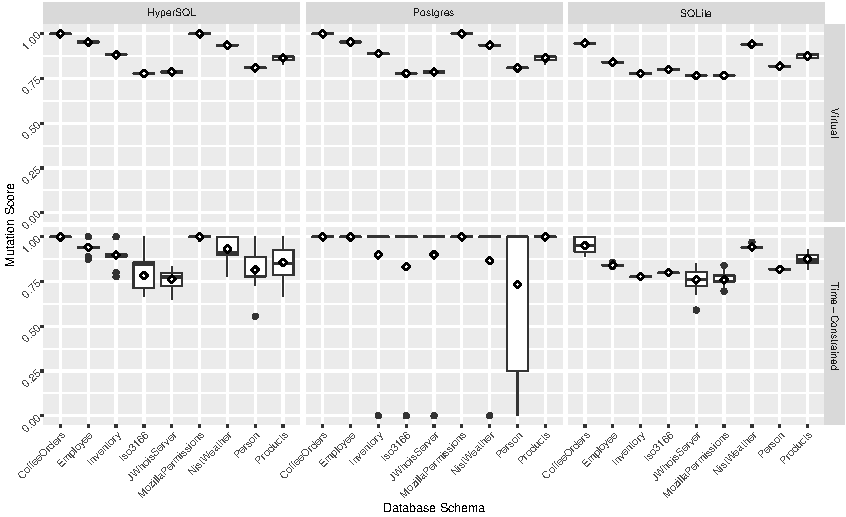
\includegraphics[scale=1.0]{graphics/graphic_bwplot_schema_mutationscore_vm_tcm.pdf}
  \caption{Box plot of the mutation score for the virtual and time-constrained mutation analysis techniques.}\label{fig:graphic_bwplot_schema_mutationscore_vm_tcm}

  % NOTE: This caption is not yet correct.

  {\small \justifying{\noindent The meaning for this box plot's elements is the same as the meaning of those described
      in the subcaption of Figure~\ref{fig:graphic_bwplot_schema_analysistime_org_vm}. Additionally, in this box plot a
      filled circle denotes an outlier and the open diamond is the mean value. Using test suites from thirty separate
      runs of the search-based test data generation method developed by McMinn \etal~\cite{McMinn2015}, this plot shows
      the variation in the mutation score for both the virtual and the time-constrained method and for all of the chosen
  relational schemas and the three database management systems. } \par}

\end{figure*}


% GRAPHIC: This is the bar chart of the number of mutants that each technique ran during mutation analysis
% NOTE: This graph was removed due to space constraints, it can be summarized in the text, I think.
% %!TEX root=ast2016.tex

\begin{figure*}[t]
  \centering
  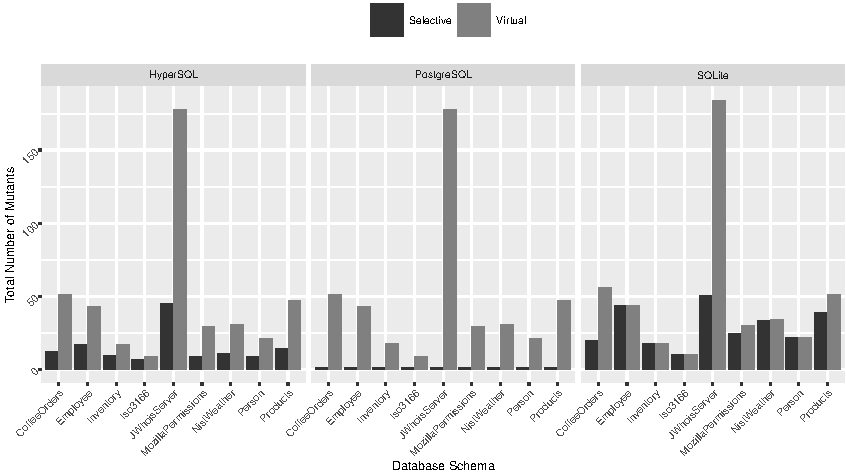
\includegraphics[scale=1.0]{graphics/graphic_barplot_schema_mutantcount_vm_tcm.pdf}
  \caption{Bar plot of the mutant count for both the virtual and time-constrained mutation analysis techniques.}
  \label{fig:graphic_barplot_schema_mutantcount_vm_tcm}

  {\small \justifying{ \noindent In this plot the height of the bar corresponds to the number of mutants subject to
      analysis by the virtual and time-constrained methods; this count is reported for all of the chosen relational
      schemas and the three database management systems. Since the time-constrained technique employs randomness to
      select mutants that can be run within a specified time limit, the height of a light grey bar is the average across
      a total of thirty runs; virtual mutation analysis is deterministic and thus the height of the dark grey bar is a
      direct count. } \par}

\end{figure*}


\inlineheading{Virtual and Time-Constrained Mutation} Since the experiments revealed that \vma~is faster than the \Original~one in $22$ out of the $27$ studied configurations --- and competitive with the DBMS-based method in the other $5$ --- it is useful to ascertain whether the presented technique might yield more accurate mutation scores in some circumstances. To this end, Figure~\ref{fig:graphic_bwplot_schema_mutationscore_vm_tcm} presents the mutation score of both the virtual approach and a time-limited analysis in which \Original~randomly analyses mutants for as long as virtual. These box plots show that the time-constrained technique results in mutation scores that are often highly variable. This result can be attributed to randomness inherent in running mutation analysis under a strict time limit that will not permit the examination of every mutant. For instance, the noticeable variability in mutation score when the Person schema is run on \Postgres~is due to the possibility of not finishing the analysis of the first mutant.

Bearing in mind that the virtual method produces mutation scores that are always equal to those achieved by the standard technique, it is also important to observe that time-constrained mutation analysis leads to overly high mutation scores.  Yet, at least for the \HyperSQL~and \SQLite~DBMSs, the box plots in Figure~\ref{fig:graphic_bwplot_schema_mutationscore_vm_tcm} suggest that the mutation scores are roughly similar for \vma~and the time-constrained method. To rigorously establish this correlation, we calculated Kendall's \taub~for the two techniques on each of the DBMSs, arriving at the values of $0.561$ (moderate), $0.132$ (low) and $0.756$ (high) for \HyperSQL, \PostgreSQL and \sqlite, respectively. These correlations suggest that virtual mutation is the best option when highly accurate scores are needed and there is limited time for mutation analysis of a database schema.

% These correlations suggest that the time-constrained mutation
% analysis of a schema for fast, in-memory databases like \HyperSQL~and \sqlite~leads to scores that respectively have a
% moderate and high correlation with the actual score. Yet, the scores produced by virtual and time-constrained mutation
% analysis on \postgres~have a low correlation. Overall, these results indicate that virtual mutation is the best option




